\documentclass{article}	
% \usepackage[
%   height=2in,      % height of the text block
%   width=7in,       % width of the text block
%   top=100pt,        % distance of the text block from the top of the page
%   headheight=48pt, % height for the header block
%   headsep=30pt,    % distance from the header block to the text block
%                % ensure an integer number of lines
%            % show the values of the parameters in the log file
% ]{geometry}

\usepackage[margin=0.75in]{geometry}
\usepackage{fancyhdr}
\usepackage{duckuments}
\usepackage{enumitem}
\usepackage{graphicx}
\usepackage{tikz}
\usepackage[OT1]{fontenc}
\usetikzlibrary{automata,positioning}
\usetikzlibrary{shapes.geometric, arrows}
\usetikzlibrary{shapes.multipart}
\usetikzlibrary{calc, arrows.meta}
\usepackage{hyperref}
\usepackage{amssymb}
\usepackage{tikz}
\usepackage{bm}
\usetikzlibrary{patterns}
\renewcommand{\familydefault}{\sfdefault}

\fancypagestyle{otherpages}{
    \fancyhf{}
    \fancyhead[LO]{MNBW2}
    \fancyhead[RO]{[MA9714]}
    \fancyfoot[RO]{Seite \thepage}
    \fancyfoot[LO]{Penguin}
}
\usepackage{amsmath}
\usepackage{lastpage} % To reference last page's number
\begin{document}
\begin{flushright}
    \includegraphics[width=2.2cm]{/home/penguin/Downloads/tum-logo/tum-logo.png} \\
\end{flushright}
\vspace{-1.7cm}
\noindent
\large 
\textcolor[HTML]{165DB1}{Mathematische Behandlung der Natur- und Wirtschaftswissenschaften 2
\\ Department Mathematics}
\vspace{5mm}
\noindent\hrule width \textwidth height 0.00001pt \relax
\normalsize
\vspace{3mm}
\section{Basics of Ordinary Differential Equations (Grundlagen: Gewöhnliche Differentialgleichungen)}
\subsection{Solving a Differential Equation}
\textbf{Case 1: Homogeneous DE}\\[2mm]
we have: 
\hspace{10mm}$i(t) = 0$ \hspace{5mm}and
\hspace{5mm}$k'(t) = \delta k(t)$ \\[2mm]
\text{Claim: solution is} $k(t)=\gamma\cdot e^{\delta t}$ \newline
\text{Set of solutions for the homogeneous DE:} $\{\gamma\cdot e^{\delta t} : \gamma \in R\}$ \\[3mm]
\textbf{Case 2: Inhomogeneous DE} \hspace{5mm} we have a general $i(t)$ 
\begin{enumerate}
    \item It is sufficient to determine (particular) solution of the Inhomogeneous DE \newline
    $K_n(t) \rightarrow$ solution for the homogeneous DE $\Rightarrow$ $K'_n (t) = \delta \cdot K_n (t)$ 
    \newline
    $K_p(t) \rightarrow$ solution for the Inhomogeneous DE $\Rightarrow$ $K'_p(t) = \delta \cdot K_p (t) + i(t)$
    \newline combining both Equations, we have: \newline
    \begin{equation*}
    \begin{split} 
    K'(t) & = K'_p(t)+K'_n(t) \\
          & = \delta \cdot K_p(t) + i(t) + \delta \cdot K_n(t) \\
          & = \delta \cdot \left(K_p(t)+K_n(t)\right) + i(t) \\
          & = \delta \cdot K(t) + i(t)
    \end{split} 
    \end{equation*}
    \item \text{Determine one solution for Inhomogeneous DE through variation of constant} \newline
    $k(t) = \gamma \cdot e^{\delta t}$ \newline
    $k(t) = c(t) \cdot e^{\delta t}$ \newline
    substituting this into the DE  \\[1mm]
    \begin{equation} k'(t) = c'(t) \cdot e^{\lambda t} + c(t) \cdot \delta e^{\delta t} \end{equation}
    \begin{equation} k'(t) = k(t) \cdot \lambda + i(t) \end{equation} 
    from (1) and (2) we have:
    \begin{equation*} c'(t) \cdot e^{-\lambda \cdot t} = i(t) \end{equation*} \newline
    Integrating both sides 
    \hspace*{30mm} \begin{equation*}c(t) = \int {i(t) \cdot e^{-\lambda t}dt} \end{equation*}
    \vspace{5mm}
\end{enumerate}
\textbf{Example:} Solving an Ordinary Differential Equation
\begin{equation*} f'(x) = 1 - x + f(x), \hspace{1mm} f(0) = 2 \end{equation*} 
\begin{enumerate} 
    \item \text{Homogeneous DE:} 
    \begin{equation*}f'(x) = f(x) \Rightarrow f(x) = \gamma \cdot e^{x} \end{equation*}
    check: \begin{equation*} f'(x) = f(x) = \gamma \cdot e^{x} - \gamma \cdot e^{x} = 0 \end{equation*}
    \item \text{Variation of constant:} 
    \begin{equation*} f(x) = c(x) \cdot e^{x} \end{equation*}
    \begin{equation*} f'(x) = c'(x) \cdot e^{x} + c(x) \cdot e^{x} \end{equation*} 
    \begin{equation*} f'(x) - f(x) = 1 - x \end{equation*}  
    Replacing $f'(x)$ and $f(x)$ with the function of $c(x)$ and $c'(x)$
    \begin{equation*} c'(x) \cdot e^{x} + c(x) \cdot e^{x} - c(x) \cdot e^{x} = 1 - x \end{equation*} 
    \begin{equation*}  c'(x) = e^{-x} \cdot (1-x) \end{equation*}
    \begin{equation*}  c(x) = \int e^{-x} \cdot (1-x) dx \end{equation*}
    \begin{equation*}  c(x) = \int e^{-x} dx - \int e^{-x} \cdot x dx \end{equation*}
    \begin{equation*}  c(x) = e^{-x} \cdot x \end{equation*}
\text{Particular solution:} \begin{equation*} f(x) = c(x) \cdot e^{x} \Rightarrow f(x) = e^{-x} \cdot x \cdot e^{x} \end{equation*}
\begin{equation*} f(x) = x \Rightarrow f'(x) = 1 \end{equation*}
    \item \text{Set of solutions:} \newline
          \begin{equation*} f(x) = x + \gamma \cdot e^{x} \end{equation*}
    \item Initial Value: \begin{equation*} f(0) = 2 \end{equation*} 
         \begin{equation*} f(0) = 0 + \gamma = 2 \Rightarrow \gamma = 2 \end{equation*}
         \begin{equation*} \rightarrow  f(x) = x + 2 \cdot e^{x} \end{equation*}
         \text{solves the initial value problem}
\end{enumerate} 
\pagestyle{otherpages}
\textbf{Note: You can also solve the Differential Equation with the help of an integrating factor}\newline Refer to this wikipedia article \href{https://en.wikipedia.org/wiki/Integrating_factor}{integrating factor} and this \href{https://www.mathcentre.ac.uk/resources/uploaded/mathcentre-ode.pdf}{text}
\\[3mm]
\hspace*{70mm} \textbf{***} 
\subsection{System of Differential Equations}
A homogeneous system of Linear Differential Equations with constant coefficients is a system of the form: \\[2mm]
\begin{equation*}\begin{pmatrix} y'_1(t) \\ \vdots \\ \vdots \\ y'_n(t) \end{pmatrix} = A \cdot \begin{pmatrix} y_1(t) \\ \vdots \\ \vdots \\ y_n(t) \end{pmatrix}, \hspace{5mm} \begin{pmatrix} y_1(0) \\ \vdots \\ \vdots \\ y_n(0) \end{pmatrix} = \begin{pmatrix} \gamma_1 \\ \vdots \\ \vdots \\ \gamma_2 \end{pmatrix}\end{equation*} \\[2mm]
\hspace*{45mm} where A $\in R$ and $\begin{pmatrix} \gamma_1 \\ \vdots \\ \vdots \\ \gamma_2 \end{pmatrix} \in R^{n} $ \\[2mm]
The key idea is that if A is a diagonal matrix, then each row is a Differential Equation that is independent of the others, solve each row separately \textbf{decoupled system}
\begin{equation*} \begin{pmatrix} y'_1(t) \\ y'_2(t) \end{pmatrix} = \begin{pmatrix} \lambda_1 & 0 \\ 0 & \lambda_2 \end{pmatrix} \begin{pmatrix} y_1(t) \\ y_2(t) \end{pmatrix}  \end{equation*}
We need a basis and a corresponding basis transformation S $\in R^{n \times n}$ such that $S^{-1}AS = D$ is diagonal \newline
Then we substitute, y = SZ $\Rightarrow Z = S^{-1}y$ \newline
The DE system, \begin{equation*} y' = A \cdot y \end{equation*} 
becomes \begin{equation*} S \cdot z = A \cdot S \cdot Z \end{equation*} 
\begin{equation*} Z' = S^{-1} \cdot A \cdot S \cdot Z = D \cdot Z \end{equation*}
Solve the new decoupled system and transform solution back through $y = SZ$ \newline
\textbf{Example:} 
\begin{equation*} \gamma'(t) = \frac{5}{2} \cdot \gamma(t) - \phi(t) \end{equation*}
\begin{equation*} \phi'(t) = \frac{-1}{4} \cdot \gamma(t) + \frac{5}{2} \phi(t) \end{equation*}
matrix form \begin{equation*} \begin{pmatrix} \gamma' \\[6pt] \phi' \end{pmatrix} = \begin{pmatrix} \dfrac{5}{2} & -1 \\[9pt] \dfrac{-1}{4} & \dfrac{5}{2} \end{pmatrix} \begin{pmatrix} \gamma \\[6pt] \phi \end{pmatrix}\end{equation*}
now, determine the eigenvalues and eigenvectors for the matrix\newline
\begin{equation*} p_A(\lambda) = \det(A-\lambda I_2) = \det\begin{pmatrix} \dfrac{5}{2} - \lambda & -1 \\[9pt] \dfrac{-1}{4} & \dfrac{5}{2} - \lambda \end{pmatrix} = {\left(\frac{5}{2}-\lambda\right)}^{2} - \frac{1}{4} = \frac{25}{4} + \lambda^{2} - 5\lambda - \frac{1}{4} = 6 + \lambda^{2} -5\lambda = (\lambda-3)(\lambda-2) \end{equation*}
The roots of the equation are $\lambda_1 = 3$ and $\lambda_2 = 2$ \newline
For the respective eigenspaces, we get \newline
\begin{equation*} eig_A(3) = \ker(A-3I_2) = \ker\begin{pmatrix} \dfrac{-1}{2} & -1 \\[9pt] \dfrac{-1}{4} & \dfrac{-1}{2}\end{pmatrix} = \ker\begin{pmatrix} \dfrac{1}{2} & -1 \\[9pt] 0 & 0\end{pmatrix} = span\begin{Bmatrix}\begin{pmatrix} -2 \\1 \end{pmatrix}\end{Bmatrix} \end{equation*}
\begin{equation*} eig_A(2) = \ker(A-2I_2) = \ker\begin{pmatrix} \dfrac{1}{2} & -1 \\[9pt] \dfrac{-1}{4} & \dfrac{1}{2}\end{pmatrix} = \ker\begin{pmatrix} \dfrac{1}{2} & -1 \\[9pt] 0 & 0\end{pmatrix} = span\begin{Bmatrix}\begin{pmatrix} 2 \\1 \end{pmatrix}\end{Bmatrix} \end{equation*}
\begin{equation*} S = \begin{pmatrix} -2 & 2 \\ 1 & 1 \end{pmatrix}\end{equation*}
\begin{equation*} S^{-1} = \frac{-1}{4}\begin{pmatrix} 1 & -2 \\ -1 & -2 \end{pmatrix}\end{equation*}
\begin{equation*} S^{-1}AS = \begin{pmatrix} 3 & 0 \\ 0 & 2 \end{pmatrix} = D \end{equation*}
Solve the system: \begin{equation*} Z' = DZ = \begin{pmatrix} 3 & 0 \\ 0 & 2 \end{pmatrix} \end{equation*}
\begin{equation*} Z_1(t) = \gamma_1 e^{3t} \end{equation*}
\begin{equation*} Z_2(t) = \gamma_2 e^{2t} \end{equation*}
\\[2mm]
\begin{equation*} \begin{pmatrix} \gamma \\[6pt] \phi  \end{pmatrix} = \begin{pmatrix} -2 & 2 \\[6pt] 1 & 1 \end{pmatrix} \begin{pmatrix} \gamma_1 e^{3t} \\[6pt] \gamma_2 e^{2t} \end{pmatrix} \end{equation*}
\begin{equation*} \gamma(t) = -2 \gamma_1 e^{3t} + 2 \gamma_2 e^{2t} \end{equation*}
\begin{equation*} \phi(t) = \gamma_1 e^{3t} \gamma_2 e^{3t} \end{equation*}
we know the initial values: $\gamma(0) = 60$ and $\phi(0) = 60$ \newline
\begin{equation*} -2\gamma_1 + 2\gamma_2 = 60\end{equation*}
\begin{equation*} \gamma_1 + \gamma_2 = 60 \end{equation*} 
solving, we get $\gamma_1 = 15$ and $\gamma_2 = 45$
\begin{equation*} \gamma(t) = -30 e^{3t} + 90 e^{2t} \end{equation*}
\begin{equation*} \phi(t) = 15 e^{3t} + 45 e^{2t} \end{equation*}
\normalsize
\pagestyle{otherpages}
\subsection*{Basics of Complex Numbers}
A complex number is represented as $Z = a + i b$ where a and b are real numbers and \begin{equation*} Re(Z)=a \end{equation*} \begin{equation*} Im(Z)=b \end{equation*}
\begin{equation*} i = \sqrt{-1} \end{equation*}
\begin{equation*} i^{2} = -1 \end{equation*}
A complex number can be represented on an argand plane with the X-axis as the real part of the complex number and the Y-part as the imaginary part of the complex number\\[2pt]
\
\subsubsection*{Algebra of Complex numbers}
Two complex numbers $Z_1 = a_1 + i b_1$ and $Z_2 = a_2 + i b_2$ can be added and subtracted by seperately adding/subtracting their real and imaginary parts. \\
Multiplication of two complex numbers,
\begin{equation*} Z_1 \cdot Z_2 = a_1 a_2 + i a_1 b_2 + i b_1 a_2 + i^{2} b_1 b_2 = a_1 a_2 + i (a_1 b_2 + b_1 a_2) - b_1 b_2  \end{equation*}
Division of two complex numbers, \\
Mulitiplying both numerator and denominator by the \textbf{conjugate} of the denominator inorder to obtain a real denominator and a complex numerator.
For example,
\begin{equation*} \frac{4+3i}{1+2i} = \frac{(4+3i)(1-2i)}{(1+2i)(1-2i)} = \frac{4-8i+3i-6i^2}{1-4i^2} = \frac{12+5i}{5} = \frac{12}{5} + i \end{equation*}
\subsection*{Complex Conjugate and absolute value}
For a complex number $Z = a + ib$, the complex conjugate is defined as $\overline{Z} = a - ib$ 
\begin{equation} Z\overline{Z} = (a+ib)(a-ib) = a^{2} - i ab + i ab + b^{2} = a^{2} + b^{2}\end{equation}
As per the definition of the absolute value of a complex number
\begin{equation} |Z| = \sqrt{a^2 + b^2} \end{equation} 
By (1) and (2), we have
\begin{equation*} Z\overline{Z} = |Z|^{2} \end{equation*}
\subsection*{Polar form and Euler's form}
Representing the complex number in the form of a $|Z|$ and argument $\phi$ 
\begin{equation*} Z = |Z| (\cos\phi+i \sin\phi)\end{equation*} is the Polar representation of a complex number
\begin{equation*} e^{i \phi} = \cos\phi + i \sin \phi \end{equation*}
Therefore, 
\begin{equation*} Z = |Z| e^{i \phi} \end{equation*} is the Euler form of the complex number 
A lot of cool stuff related to \href{https://www.youtube.com/playlist?list=PLJbzH0qGCsyrO7lUmdEQAzJInNlwwUgp0}{complex number} on this playlist. Not required for economic aspects though.
\section{Eigenvectors and Eigenalues}
$S \in R^{n\times n}$ \\
$A \in R^{n \times n}$ \\
$S^{-1}AS = D$ diagonal matrix, tranformation matrix \\
Is there a basis transformation? \\ 
$\lambda \in R$ is called an eigenvalue of A if there exists a vector $v \neq \phi$ such that \begin{equation*} A \cdot v = \lambda \cdot v \end{equation*}
Any such vector v in this case would be called an eigen vector of A for the eigen value $\lambda$
\textbf{Gaussian Reformulation:} Determination of the eigenvalues and eigenvectors. \\
$\lambda$ is an eigenvalue of A if there $v\neq\phi$ with $A\cdot v = \lambda \cdot v$
\begin{equation*}
    \Leftrightarrow A\cdot v - \lambda \cdot v = 0 \end{equation*}
\begin{equation*}\Leftrightarrow (A-\lambda E_n) \cdot v = 0 \end{equation*}
\begin{equation*} \Leftrightarrow v \in \ker(A\cdot\lambda E_n) \end{equation*}
\begin{equation*}\Leftrightarrow (A-\lambda E_n) \text{  is not invertible} \end{equation*}
\begin{equation*} \Leftrightarrow \det(A-\lambda E_n) = 0 
\end{equation*} \\[2pt]
The \textbf{characteristic polynomial} $p_A(\lambda)$ is defined as the determinant $\det(A-\lambda E_n)$ \begin{equation*} p_A(\lambda) = \det(A-\lambda E_n) \end{equation*} \\ and the kernel $\ker(A-\lambda E_n)$ is called the \textbf{eigenspace of A for the eigenvalue $\lambda$} and written as \begin{equation*} eig_A(\lambda) = \ker(A-\lambda E_n) \end{equation*}
The idea to solve each and every problem here is quite simple,
\begin{enumerate}
    \item First of all, determine the \textbf{characteristic polynomial} [Diagonalized matrix S is the matrix with the eigenspaces of the respective eigenvalues]
    \item Find the roots of the characteristic polynomial, these are the eigenvalues of A
    \item For each eigenvalue of A, determine the eigenspace by solving the linear equation system \\ $(A-\lambda E_n) \cdot v = 0$ 
\end{enumerate}
\subsection{Diagonalization using complex numbers} 
characterizing which matrices can be transformed into diagonal form, ie possess an eigenvector basis. \\
A matrix $A\in R^{n\times n}$ is called \textbf{diagonalizable} if there is a basis of $R^{n}$ that consists of eigenvectors of A\\[2pt]
\underline{NOTE:} For each eigenvalue $\rightarrow$ there is at least one eigenvector ie. $\dim(eig_A(\lambda)) \geq 1$ for each eigenvalue $\lambda$ 
$\Rightarrow$ if A possesses n distinct eigenvalue, then there are at least n eigenvectors \\
\begin{equation*} p_A(\lambda) = {(\lambda - \lambda*)}^k \cdot g(\lambda) \text{   and  } g(\lambda*) \neq 0 \end{equation*}
Then k is called the \textbf{algebraic multiplicity} of $\lambda*$ and $\dim(eig_A(\lambda*))$ is called the geometric mutliplicity of $\lambda*$
\begin{enumerate}
    \item Algebraic mulitplicity $\geq$ Geometric mulitplicity
    \item For pairwise distinct eigenvalues of A with corresponding eigenvectors- the set $\{v_1, \dots, v_r\}$ is linearly independent
    \item For a matrix to be diagonalizable, the algebraic and the geometric mulitplicity have to be equal for every eigenvalue of A 
\end{enumerate}
Proving (2) is pretty simple as you can simply use the principle of induction after solving it for 2 eigenvalues and their corresponding eigenvectors
\\ If roots are complex, we can use the Euler's formula \begin{equation*} e^{i \phi} = \cos\phi + i \sin \phi \end{equation*}
what if the matrix cannot be diagonalized? \textbf{JORDAN NORMAL FORM} as \href{https://en.wikipedia.org/wiki/Jordan_normal_form}{generalizations} and refer \href{https://shorturl.at/9Vxni}{for} Inhomogeneous Differential Equation system 
\\\url{https://people.math.harvard.edu/~knill/teaching/math19b_2011/handouts/lecture29.pdf} for a recap
\subsection{Predator-Prey Model}
squirrels-hawks $\rightarrow$ The growth of hawk population depends on availability of squirrels and vice-versa. [Fewer hawks $\rightarrow$ higher the growth rate of squirrels]
\\ Model this through DE system:
\begin{equation*} h'(t) = s(t) - 12 \text{ and } h(0) = 6\end{equation*}
\begin{equation*} s'(t) = -h(t) \text{  and  } s(0) = 20 \end{equation*}
\begin{enumerate} 
    \item \underline{get rid of constants:} define a new system \\
    \begin{equation*} y_1(t) = h(t) - 10 = -s'(t) \text{    and    } y_1(0) = h(0) - 10 = -4\end{equation*}
    \begin{equation*} y_2(t) = s(t) - 12 = h'(t) \text{   and   }  y_2(0) = s(0) - 12 = 8 \end{equation*}
    \begin{equation*} \Rightarrow y_1'(t) = h'(t) = s(t) - 12 = y_2(t)  \end{equation*}
    \begin{equation*} \Rightarrow y_2'(t) = -h(t) + 10 \end{equation*} 
    \text{new system without constants:} 
    \begin{equation*} \begin{pmatrix} y_1'(t) \\ y_2'(t) \end{pmatrix} = \begin{pmatrix} 0 & 1 \\ -1 & 0 \end{pmatrix} \begin{pmatrix} y_1(t) \\ y_2(t) \end{pmatrix} \mid \begin{pmatrix} y_1(0) \\ y_2(0) \end{pmatrix} = \begin{pmatrix} -4 \\ 8 \end{pmatrix} \end{equation*} 
    \item \underline{Diagonalize the matrix A} [find eigenvalues and the corresponding eigenvectors then form the S matrix]\begin{equation*} A = \begin{pmatrix} 0 & 1 \\ -1 & 0 \end{pmatrix} \end{equation*}
    not showing the calculations but the eigenvectors are $+i$, $-i$ and eigenvectors are $\begin{pmatrix} 1 \\ i \end{pmatrix}$ and $\begin{pmatrix} 1 \\ -i \end{pmatrix}$ so the required S matrix is $\begin{pmatrix} 1 & 1 \\ i & -i \end{pmatrix}$ \\
    \begin{equation*} S^{-1}AS = \begin{pmatrix} i & 0 \\ 0 & -i \end{pmatrix} \end{equation*}
    \item \underline{consider the decoupled system after substitution} $y=SZ$ \\
    \begin{equation*} Z'(t) = \begin{pmatrix} i & 0 \\ 0 & i \end{pmatrix} Z(t)\end{equation*}
    $\Rightarrow$
    \begin{equation*} Z_1'(t) = i\cdot Z_1(t) \Rightarrow Z_1(t) = \gamma_1 \cdot e^{i t} \end{equation*}
    \begin{equation*} Z_2'(t) = -i \cdot Z_2(t) \Rightarrow Z_2(t) = \gamma_2 \cdot e^{-i t} \end{equation*}
    \item \underline{determine y = SZ:} \begin{equation*} y(t) = \begin{pmatrix} 1 & 1 \\ i & -i \end{pmatrix} \begin{pmatrix} \gamma_1 e^{i t} \\ \gamma_2 e^{-i t} \end{pmatrix}\end{equation*}  
    $\Rightarrow$
    \begin{equation*} y_1(t) = \gamma_1 e^{i t} + \gamma_2 e^{-i t} \end{equation*}
    \begin{equation*} y_2(t) = \gamma_2 i e^{i t} - \gamma_2 i e^{-i t} \end{equation*} 
    \item \underline{Determine $\gamma_1$, $\gamma_2$ through initial values:}
    \begin{equation*} y_1(0) = -4 = \gamma_1 \cdot 1 + \gamma_2 \cdot 1 \end{equation*}
    \begin{equation*} y_2(0) = 8 = \gamma_1 \cdot i \cdot 1 - \gamma_2 \cdot i \cdot 1 \end{equation*}
    \begin{equation*} \rightarrow \begin{pmatrix} 1 & 1 &\bigm| & -4 \\  i & -i &\bigm| & 8  \end{pmatrix} \rightarrow \begin{pmatrix} 1 & 1 &\bigm| & -4 \\ 0 & -2i &\bigm| & 8+4i \end{pmatrix} \end{equation*}
    \begin{equation*} (-2i) \gamma_2  = 8 + 4 i \end{equation*}
    \begin{equation*} \Leftrightarrow \gamma_2 = 4i - 2 = -2 + 4i \end{equation*} 
    \begin{equation*} \Rightarrow \gamma_1 = -4 - \gamma_2 = -2 - 4i \end{equation*}
    \textbf{Solutions:}
    \begin{equation*} y_1(t) = (-2 - 4i) e^{i t} + (-2 + 4i) e^{-i t} \end{equation*} 
    \begin{equation*} y_2(t) = (4 - 2i) e^{i t} + (4 + 2i) e^{-i t} \end{equation*}
    \item \underline{Use Euler's Formula:} replace $e^{i t}$ and $e^{-i t}$ with $cis\theta$ terms
    \begin{equation*} y_1(t) = -4\cos t + 8\sin t \mid h(t) = -4\cos t + 8\sin t + 10\end{equation*}
    \begin{equation*} y_2(t) = 8\cos t + 4\sin t \mid s(t) = 8\cos t + 4\sin t + 12 \end{equation*}
\end{enumerate} \vspace{10mm}
\section{Multivariable Calculus}
\subsection{Fundamentals}
\textbf{Definition:} Let $f : X \rightarrow Y$ be a function with $ X \subseteq \mathbb{R}^{n} $ (domain) and $ Y \subseteq \mathbb{R}^{n} $ (codomain) for $m, n \in \mathbb{N}$ \\
The graph of $f$ is the set 
\begin{equation*} graph(f) = \left\{\begin{pmatrix} x \\ f(x)\end{pmatrix} :  x \in X \right\} \end{equation*}
A function of two variables assigns a real number to each point in a subset of $\mathbb{R}^2$. For example,
\[
f(x, y) = x^2 + y^2
\]
defines a function over $\mathbb{R}^2$.
The \textbf{domain} of a multivariable function is the set of all input values for which the function is defined. The \textbf{range} is the set of all output values.
Example: For $f(x, y) = \sqrt{1 - x^2 - y^2}$, the domain is the unit disk:
\[
D = \{(x, y) \in \mathbb{R}^2 : x^2 + y^2 \leq 1\}
\]
\textbf{Definition:} Let $f : X \rightarrow \mathbb{R}$, $ X \subseteq \mathbb{R}^{n} $ be a function and let $\gamma \in \mathbb{R}$ \\ 
The set 
\begin{equation*} L_{f} (\gamma) := \left\{x \in X : f(x) = \gamma \right\}\end{equation*} is called the \underline{level set of $f$ for level $\gamma$}
\newpage 
\subsection{Basic Topology}
\subsubsection{Open Balls and $\delta$-Neighborhoods}
Let $x^{*} \in \mathbb{R}^n$, $\delta > 0$. Then the $\delta$-neighborhood of $x^{*}$ is the set
\[
N_{\delta} (x^{*}) := \left\{x \in \mathbb{R}^{n}: ||x - x^{*}|| < \delta\right\}
\]
for some $\delta > 0$. $N_{\delta}$ is called \textbf{open ball of radius $\delta$ around $x^{*}$ and sometimes denoted by $B_{\delta}(x^{*}$)} 

\subsubsection{Interior Points}
A point $x \in A \subseteq \mathbb{R}^n$ is called an \textbf{interior point} of $A$ if there exists a $\delta > 0$ such that:
\[
N_{\delta} (x*) \subseteq X
\]
The set of all interior points of $X$ is called the \textbf{interior} of $X$, denoted $\operatorname{int}(X)$.

\subsubsection{Boundary Points}
A point $x \in \mathbb{R}^n$ is a \textbf{boundary point} of a set $A$ if every $\delta$-neighborhood of $x$ intersects both $X$ and its complement (not in $X$):
\[
\forall \delta > 0,\ N_\delta(x^{*}) \cap X \neq \emptyset \quad \text{and} \quad N_\delta(x^{*}) \cap (\mathbb{R}^n \setminus X) \neq \emptyset
\]
The set of all boundary points is called the \textbf{boundary} of $X$, denoted $bd(X)$ or $\partial X$.
\\ 
The set $cl(X) := X \cup bd(X)$ is called \textbf{closure} of $X$ (sometimes written $\bar{X}$)
\subsubsection{Closure of a Set}
The \textbf{closure} of a set $X$, denoted $\overline{X}$, is the union of $X$ and its accumulation points. Equivalently,
\[
\overline{X} = X \cup \partial X
\]
\subsubsection{Open and Closed Sets}
\begin{enumerate} \item A set $A$ is \textbf{open} if all its points are interior points, i.e., $A = \operatorname{int}(A)$.
\item A set is \textbf{closed} if it contains all its boundary points.
\end{enumerate}
\subsubsection{Accumulation (Limit) Points}
A point $x$ is an \textbf{accumulation point} (or limit point) of a set $X$ if every neighborhood of $x$ contains at least one point of $X$ different from $x$:
\[
\forall \delta > 0, \quad (B_\delta(x) \setminus \{x\}) \cap X \neq \emptyset
\]
\newpage 
The set $X$ is called 
\begin{enumerate}
    \item \textbf{open} if $X = int(X)$
    \item \textbf{closed} if $\mathbb{R} \setminus X$ is open 
    \item \textbf{bounded} if there is some $\delta > 0$ such that $X \subseteq N_{\delta}(0)$
    \item \textbf{compact} if it is closed and bounded.
\end{enumerate} \vspace{10mm}
    1. $\delta$-Neighborhood (Open Ball)
\begin{center}
    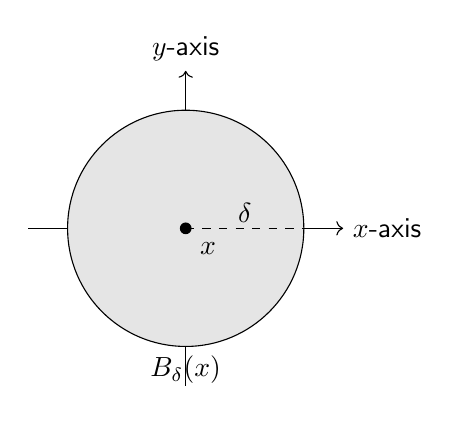
\begin{tikzpicture}
      \draw[->] (-2,0) -- (2,0) node[right] {$x$-axis};
      \draw[->] (0,-2) -- (0,2) node[above] {$y$-axis};
    
      \filldraw[fill=gray!20, draw=black] (0,0) circle (1.5);
      \node at (0,0) [circle,fill,inner sep=1.5pt,label=below right:$x$] {};
    
      \draw[dashed] (0,0) -- (1.5,0);
      \node at (0.75,0.2) {$\delta$};
      \node at (0,-1.8) {$B_\delta(x)$};
    \end{tikzpicture}
    \end{center}
    \vspace{5mm}
    2. Interior Point
    \begin{center}
    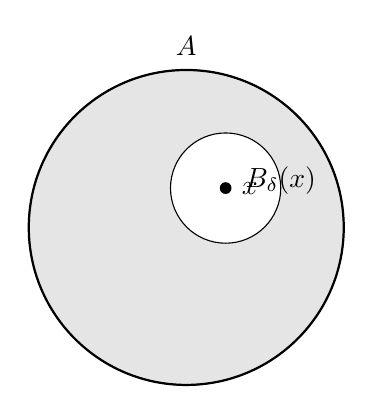
\begin{tikzpicture}
      \draw[fill=gray!20] (0,0) circle (2);
      \draw[thick] (0,0) circle (2);
      \node at (0,2.3) {$A$};
    
      \filldraw[fill=white,draw=black] (0.5,0.5) circle (0.7);
      \node at (0.5,0.5) [circle,fill,inner sep=1.5pt,label=right:$x$] {};
      \node at (1.2,0.6) {$B_\delta(x)$};
    \end{tikzpicture}
    \end{center}
    \vspace{5mm}
    3. Boundary Point
    \begin{center}
    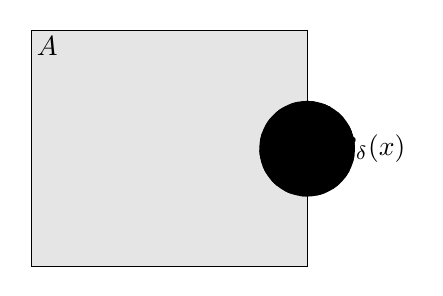
\begin{tikzpicture}
      \draw[fill=gray!20] (-2,-1) rectangle (1.5,2);
      \node at (-1.8,1.8) {$A$};
    
      \filldraw[draw=black] (1.5,0.5) circle (0.6);
      \node at (1.5,0.5) [circle,fill,inner sep=1.5pt,label=above:$x$] {};
      \node at (2.3,0.5) {$B_\delta(x)$};
    
      \draw[dashed] (1.5,0.5) circle (0.6);
    \end{tikzpicture}
    \end{center}
    \vspace{50mm}
    4. Closed Set
    \begin{center}
    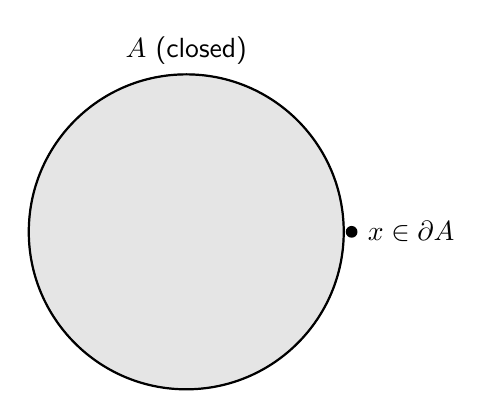
\begin{tikzpicture}
      \draw[fill=gray!20] (0,0) circle (2);
      \draw[thick] (0,0) circle (2);
      \node at (0,2.3) {$A$ (closed)};
      \node at (2.1,0) [circle,fill,inner sep=1.5pt,label=right:$x \in \partial A$] {};
    \end{tikzpicture}
\end{center}
    \vspace{5mm}
    5. Open Set
    \begin{center}
    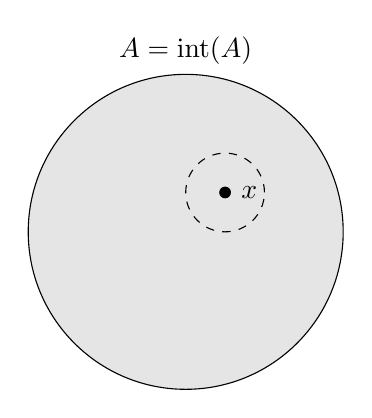
\begin{tikzpicture}
      \draw[fill=gray!20] (0,0) circle (2);
      \node at (0,2.3) {$A = \operatorname{int}(A)$};
      \node at (0.5,0.5) [circle,fill,inner sep=1.5pt,label=right:$x$] {};
      \draw[dashed] (0.5,0.5) circle (0.5);
    \end{tikzpicture}
\end{center} \vspace{10mm}
\subsection{Sequences and Limits}
A function in $f : \mathbb{N}_{0} \rightarrow \mathbb{R}^n$ is called a \textbf{sequence} in $\mathbb{R}^{n}$ with $a_k := f(k)$ such a sequence is usually \\ denoted as $(a_k)_{k \in \mathbb{N}_{0}}$ or just $(a_k)_{\mathbb{N}_{0}}$ 
\\
A sequence $(a_k)_{\mathbb{N}}$ is called \textbf{convergent} if there exists a vector $a \in \mathbb{R}^n$ such that
\[
\forall \varepsilon > 0, \ \exists N \in \mathbb{N} \text{ such that } ||a_k - a|| \rightarrow 0 
\]
as $k \rightarrow \infty$. The vector a is called the \textbf{limit of $(a_k)_{\mathbb{N}}$} and is denoted by \begin{equation*} a = \lim a_k\end{equation*}
$(a_k)_{\mathbb{N}}$ is convergent with limit $a$ if and only for $i = 1, \dots, n$ the following holds:
\begin{enumerate}
    \item the sequence $(\alpha_ik)_{k \in \mathbb{N}}$ is convergent
    \item $\lim_{k} \alpha_{ik} = \alpha_{i}$
\end{enumerate} \newpage
\textbf{Definitions}
\begin{enumerate}
\item A sequence $\{a_k\} \subset \mathbb{R}^n$ is \textbf{bounded} if the set $\left\{a_k : k \in \mathbb{N}_{0}\right\}$ is bounded
\item Let $(a_k)_{\mathbb{N}_{0}}$ be a sequence and $f : \mathbb{N}_{0} \rightarrow \mathbb{N}_{0}$ be strictly increasing, i.e. for $p > q \implies f(p) > f(q)$. \\ Then the sequence $(a'_k)_{\mathbb{N}_{0}}$ defined as $a'_k = a_{f(k)}$ is called a \textbf{subsequence} of $(a_k)_{\mathbb{N}_{0}}$ 
\item The limit of a convergent subsequence of some sequence $(a_k)_{\mathbb{N}_{0}}$ is called the \textbf{accumulation point} of $(a_k)_{\mathbb{N}_{0}}$ 
\end{enumerate}
\subsubsection{Bolzano-Weierstrass Theorem}
\textbf{Theorem:} Every bounded sequence in $\mathbb{R}^n$ has a convergent subsequence. (i.e. at least one accumulation point) \\
in particular, if $X$ is a compact set and  $(a_k)_{\mathbb{N}_{0}}$ is a subsequence in $X$, then  $(a_k)_{\mathbb{N}}$ has a convergent subsequence with limit in $X$.
\\ 
\textit{Idea of Proof:} Use the fact that $\mathbb{R}^n$ is a product of complete metric spaces, and apply the one-dimensional Bolzano-Weierstrass theorem component-wise to extract a convergent subsequence.
\vspace{10mm}
\subsection{Continuity}

\textbf{Definition:}\\
Let \( X \subseteq \mathbb{R}^m \), \( f: X \rightarrow \mathbb{R}^m \) and \( x^* \in X \).

\begin{enumerate}
    \item[(3)] \(\alpha \in \mathbb{R}^m\) is called the limit of \( f \) for \( x \rightarrow x^* \) if the following holds:
    
    For every sequence \((a_k)_{k \in \mathbb{N}}\) in \( X \) that converges to \( x^* \), the sequence \((f(a_k))_{k \in \mathbb{N}}\) converges to \(\alpha\).
    
    \[
    \lim_{x \rightarrow x^*} f(x) = \alpha
    \]
    
    \item[(2)] \( f \) is called continuous in \( x^* \) if 
    
    \[
    \lim_{x \rightarrow x^*} f(x) = f(x^*).
    \]
    
    \item[(3)] \( f \) is called continuous on \( X \) if \( f \) is continuous at every point \( x^* \in X \).
\end{enumerate}

\subsubsection{Theorem:}
Let \( X \subseteq \mathbb{R}^m \), \( f: X \rightarrow \mathbb{R}^m \) and \( g: X \rightarrow \mathbb{R} \) be continuous on \( X \), and let \( \alpha \in \mathbb{R} \). Then the following are true:

\begin{enumerate}
    \item[(1)] \( f + g \), \( \alpha f \), and \( f \cdot g \) are continuous on \( X \).
    
    \item[(2)] \(\frac{f}{g}\) is continuous on \( X \setminus \{ x \in X : g(x) = 0 \}\).
    
    \(\frac{f}{\alpha}\) is continuous for \( \alpha \neq 0 \).
    
    \item[(3)] Let \( h: \mathbb{R}^k \rightarrow X \) be continuous, then \( f \circ h \) is continuous.
    
    \item[(4)] If 
    \[
    f(x) = \begin{pmatrix}
    f_1(x) \\
    \vdots \\
    f_m(x)
    \end{pmatrix},
    \]
    then \( f \) is continuous on \( X \) if and only if all \( f_i: X \rightarrow \mathbb{R} \) are continuous on \( X \).
\end{enumerate}

\subsubsection*{Example:}
\[
f(x_1, x_2) := \begin{pmatrix}
x_1 \cos(x_2) \\
e^{x_1 + x_2} - 1
\end{pmatrix}, \quad f: \mathbb{R}^2 \rightarrow \mathbb{R}^2.
\]

Then \( f \) is continuous:

\begin{enumerate}
    \item[(1)] \( f \) is continuous if and only if both coordinate functions are continuous:
    \[
    f_1(x_1, x_2) = x_1 \cos(x_2), \quad f_2(x_1, x_2) = e^{x_1 + x_2} - 1.
    \]
    
    \item[(2)] \( f_1 \) is a product of continuous functions, hence continuous.
    
    \item[(3)] \( f_2 \) is the sum of continuous functions. The term \( e^{x_1 + x_2} \) is continuous as it is a composition of continuous functions.
    
    \(\Rightarrow f_2 \) is continuous.
\end{enumerate}

\subsubsection*{Definition:}
A multivariate polynomial is a function \( p: \mathbb{R}^n \rightarrow \mathbb{R} \) of the form:
\[
p(x) = \sum_{I} a_I x^I,
\]
where \( I \) is a multi-index and \( a_I \in \mathbb{R} \).

\subsubsection*{Example:}
\[
p(x_1, x_2, x_3) = 2x_1^2 + 4x_2^3 + 8x_3^4.
\]

Multivariate polynomials are continuous on \( \mathbb{R}^n \).

\begin{enumerate}
    \item[(1)] Sum of simple functions (monomials).
    \item[(2)] Each monomial is a product of constants and univariate monomials.
    \item[(3)] Products and sums of continuous functions are continuous.
\end{enumerate}

\subsubsection{Theorem:}
Let \( X \subseteq \mathbb{R}^n \), \( f: X \rightarrow \mathbb{R}^m \). Then \( f \) is continuous if and only if:

\begin{enumerate}
    \item[(i)] For any open set \( Y \subseteq \mathbb{R}^m \), the preimage \( f^{-1}(Y) \) is open in \( X \).
    \item[(ii)] For every closed set \( Y \subseteq \mathbb{R}^m \), the preimage \( f^{-1}(Y) \) is closed in \( X \).
\end{enumerate}

\subsubsection{Theorem:}
Let \( X \subseteq \mathbb{R}^n \), \( f: X \rightarrow \mathbb{R}^m \) continuous. If \( X \) is compact, then \( f(X) \) is also compact (closed and bounded).

This implies: For compact \( X \subseteq \mathbb{R}^n \) with \( X \neq \emptyset \) and continuous \( f: X \rightarrow \mathbb{R} \), the function \( f \) attains its minimum and maximum on \( X \).
\vspace{10mm}
\subsubsection*{An Example and a Warning}

Let \( f: X \rightarrow \mathbb{R} \), \( X \subseteq \mathbb{R}^n \), be a multivariate function.

\[
f(x_1, x_2) = x_1^2 + x_2^2, \quad x_1 \geq x_2.
\]

We can define "directional sections" to obtain one-dimensional traces from \( f \):

\begin{itemize}
    \item Choose a direction \( d \in \mathbb{R}^n \setminus \{0\} \).
    \item Consider the function \( f_d \) obtained by restricting \( f \) to the line in the direction of \( d \):
    
    Line: \( \{0 + \lambda d : \lambda \in \mathbb{R}\} \) \\
    \( f_d: \mathbb{R} \rightarrow \mathbb{R} \) \\
    \( f_d(\lambda) = f(0 + \lambda d) \).
\end{itemize}

If \( f \) is continuous, then all directional sections are also continuous. However, the converse is not generally true. Even if all \( f_d \) for all possible directions are continuous, the function \( f \) can still be discontinuous.

\subsubsection*{Example}

\[
f: \mathbb{R}^2 \rightarrow \mathbb{R}, \quad f(x_1, x_2) := 
\begin{cases} 
\frac{x_1^2 \cdot x_2}{x_1^4 + x_2^2}, & x \neq (0, 0) \\ 
0, & x = (0, 0) 
\end{cases}
\]

Is \( f \) continuous at \( (0, 0) \)?

Let \( d \in \mathbb{R}^2 \setminus \{0\} \) be an arbitrary direction. We consider \( f_d: \mathbb{R} \rightarrow \mathbb{R} \),

\[
f_d(\lambda) = f(0 + \lambda d) = f(\lambda d_1, \lambda d_2).
\]

\[
f_d(\lambda) = 
\begin{cases} 
\frac{\lambda^3 d_1^2 d_2}{\lambda^4 d_1^4 + \lambda^2 d_2^2} = \frac{\lambda d_1^2 d_2}{\lambda^2 d_1^4 + d_2^2}, & \lambda \neq 0 \\ 
0, & \lambda = 0 
\end{cases}
\]

\begin{itemize}
    \item For \( d_2 = 0 \), \( f_d(\lambda) = 0 \) for all \( \lambda \), so \( f_d \) is continuous.
    \item For \( d_2 \neq 0 \), \( \lim_{\lambda \to 0} f_d(\lambda) = 0 = f_d(0) \), so \( f_d \) is continuous.
\end{itemize}

Thus, all directional sections \( f_d \) are continuous. However, consider the sequence \( a_k = \left( \frac{1}{k}, \frac{1}{k^2} \right) \):

\[
f(a_k) = \frac{\left( \frac{1}{k} \right)^2 \cdot \left( \frac{1}{k^2} \right)}{\left( \frac{1}{k} \right)^4 + \left( \frac{1}{k^2} \right)^2} = \frac{\frac{1}{k^4}}{\frac{1}{k^4} + \frac{1}{k^4}} = \frac{1}{2}.
\]

But \( f(0, 0) = 0 \), so \( \lim_{k \to \infty} f(a_k) = \frac{1}{2} \neq f(0, 0) \). Therefore, \( f \) is not continuous at \( (0, 0) \).
\newpage
\subsection{Partial Derivatives}
Let \( X \subseteq \mathbb{R}^n \), \( f: X \to \mathbb{R} \), and consider "directional cross-sections". For a direction \( d \in \mathbb{R}^n \setminus \{0\} \) and a point \( x^* \in \text{int}(X) \), define the function:
\[ f_d: \mathbb{R} \to \mathbb{R}, \quad f_d(\lambda) := f(x^* + \lambda d). \]
This represents \( f \) along the line through \( x^* \) in direction \( d \).

In particular, we can choose coordinate axes as directions, leading to partial functions:
\[ f_i(\lambda) := f(x^* + \lambda e_i), \]
where \( e_i \) is the \( i \)-th standard basis vector.

\subsection*{Example:}
Consider \( f: \mathbb{R}^2 \to \mathbb{R} \) defined by:
\[ f(x_1, x_2) = 7 - x_1^2 - x_2^2 + 3x_1x_2, \quad x^* = (0, 0). \]

\begin{itemize}
    \item[(7)] For directions \( e_1 \) and \( e_2 \):
    \[ f_1(\lambda) = f(\lambda, 0) = 7 - \lambda^2, \]
    \[ f_2(\lambda) = f(0, \lambda) = 7 - \lambda^2. \]
    Along these axes, \( f \) attains a maximum at \( x^* = (0, 0) \).

    \item[(8)] For direction \( d = (1, 1) \):
    \[ f_d(\lambda) = f(\lambda, \lambda) = 7 - \lambda^2 - \lambda^2 + 3\lambda^2 = 7 + \lambda^2. \]
    Here, \( f \) attains a minimum at \( x^* = (0, 0) \) along this line.
\end{itemize}

This shows that one-dimensional cross-sections may not capture all characteristics of a multivariate function.

\subsection*{Definition: Partial Differentiability}

Let \( X \subseteq \mathbb{R}^n \), \( f: X \to \mathbb{R} \), and \( x^* \in \text{int}(X) \).

\begin{itemize}
    \item[(1)] The function \( f \) is \textit{partially differentiable} at \( x^* \) with respect to \( x_i \) if the function:
    \[ g(\lambda) = f(x^* + \lambda e_i) = f(x_1^*, \dots, x_{i-1}^*, x_i^* + \lambda, x_{i+1}^*, \dots, x_n^*), \]
    is differentiable at \( \lambda = 0 \). The partial derivative is then:
    \[ g'(0) = \frac{\partial f}{\partial x_i}(x^*) = \partial_i f(x^*). \]

    \item[(2)] The function \( f \) is \textit{partially differentiable} at \( x^* \) if all partial derivatives \( \frac{\partial f}{\partial x_i}(x^*) \) exist. The \textit{gradient} of \( f \) at \( x^* \) is:
    \[ \nabla f(x^*) = \left( \frac{\partial f}{\partial x_1}(x^*), \dots, \frac{\partial f}{\partial x_n}(x^*) \right). \]

    \item[(3)] Higher-order partial derivatives are defined recursively:
    \[ \frac{\partial^2 f}{\partial x_i \partial x_j}(x^*) = \frac{\partial}{\partial x_i} \left( \frac{\partial f}{\partial x_j} \right)(x^*). \]

    \item[(4)] The \textit{Hessian matrix} of \( f \) at \( x^* \) is the matrix of second-order partial derivatives:
    \[ H_f(x^*) = D^2 f(x^*) = \left( \frac{\partial^2 f}{\partial x_i \partial x_j}(x^*) \right)_{i,j=1}^n. \]
\end{itemize}

\subsection{Directional Derivatives}

Partial derivatives describe the behavior of a function along lines parallel to the coordinate axes. But what about general directions?

\subsubsection*{Definition}

Let \( X \subseteq \mathbb{R}^n \), \( f: X \rightarrow \mathbb{R} \), and \( x^* \in \text{int}(X) \). 

For a direction \( v \in \mathbb{R}^n \setminus \{0\} \), choose \( \delta > 0 \) such that the neighborhood \( N_\delta(x^*) \subseteq X \). Define the function:
\[ g: (-\delta, \delta) \rightarrow \mathbb{R}, \quad g(\lambda) = f(x^* + \lambda v). \]

If \( g \) is differentiable at \( \lambda = 0 \), then \( g'(0) \) is called the \textit{directional derivative} of \( f \) at \( x^* \) in direction \( v \), denoted by:
\[ g'(0) = \partial_v f(x^*) = D_v f(x^*). \]

\subsubsection*{Example}

Consider \( f: \mathbb{R}^2 \rightarrow \mathbb{R} \) defined by:
\[
f(x_1, x_2) = 
\begin{cases} 
\frac{x_1^2 x_2}{x_1^4 + x_2^2}, & (x_1, x_2) \neq (0, 0) \\ 
0, & (x_1, x_2) = (0, 0) 
\end{cases}
\]

This function is not continuous at \( (0, 0) \), but it is continuous along every line through \( (0, 0) \). 

\subsubsection*{Directional Derivatives at \( (0, 0) \)}

For a direction \( v = \begin{pmatrix} v_1 \\ v_2 \end{pmatrix} \neq \begin{pmatrix} 0 \\ 0 \end{pmatrix} \), define:
\[
g(\lambda) = f(0 + \lambda v) = f(\lambda v_1, \lambda v_2) = 
\begin{cases} 
\frac{\lambda^3 v_1^2 v_2}{\lambda^4 v_1^4 + \lambda^2 v_2^2} = \frac{\lambda v_1^2 v_2}{\lambda^2 v_1^4 + v_2^2}, & \lambda \neq 0 \\ 
0, & \lambda = 0 
\end{cases}
\]

The difference quotient is:
\[
\frac{g(\lambda) - g(0)}{\lambda - 0} = 
\begin{cases} 
\frac{v_1^2 v_2}{\lambda^2 v_1^4 + v_2^2}, & \lambda \neq 0 \\ 
0, & \lambda = 0 
\end{cases}
\]

Taking the limit as \( \lambda \to 0 \):
\[
\lim_{\lambda \to 0} \frac{g(\lambda) - g(0)}{\lambda} = 
\begin{cases} 
0, & v_2 = 0 \\ 
\frac{v_1^2}{v_2}, & v_2 \neq 0 
\end{cases}
\]

\subsubsection*{Conclusion}

All directional derivatives of \( f \) at \( (0, 0) \) exist. However, this does not imply continuity at \( (0, 0) \), as shown by the earlier example. 

This demonstrates that even if a function has directional derivatives in all directions, it may still fail to be continuous at a point.

\subsubsection*{Economic Application of Multivariable Functions}
Keynes' Consumption Formula
\begin{equation*} e = c_0 + \beta \cdot I + \varepsilon_i \end{equation*}
Minimizing $\sum \varepsilon_i^{2}$ (Least Squares Regression)\\[5mm]
Cobb-Douglas Production Function (Economics I)
\begin{equation*} Y = \alpha \cdot L^{b} \cdot K^{a} \end{equation*}
our objective is to minimize $f:\mathbb{R}^3 \rightarrow \mathbb{R}$ \newpage
\section{Total Differentiability}
Let \( X \subseteq \mathbb{R}^n \) be open, \( f: X \rightarrow \mathbb{R} \), and \( x^* \in X \).

The function \( f \) is called \textit{(totally) differentiable} at \( x^* \) if there exists a vector \( g \in \mathbb{R}^n \) and a function \( r: N_\delta(0) \rightarrow \mathbb{R} \) (for some \(\delta\)-neighborhood of \( 0 \)) such that:

\[
f(x) = f(x^*) + g^T(x - x^*) + r(x - x^*)
\]

with the property:

\[
\lim_{x \to x^*} \frac{r(x - x^*)}{\|x - x^*\|} = 0.
\]

\subsubsection*{Interpretation}
\begin{itemize}
    \item The vector \( g \) provides a linear approximation to \( f \) at \( x^* \).
    \item Locally (around \( x^* \)), the approximation is "good", meaning the error term \( r \) tends to 0 faster than the distance between \( x \) and \( x^* \) as \( x \to x^* \).
    \item This implies the error is small compared to \( \|x - x^*\| \).
\end{itemize}

\subsubsection*{Notation}
\[
g^T = Df(x^*) \quad \text{is called the derivative of } f \text{ at } x^*
\]
\[
= f'(x^*)
\]

\subsection*{Total Differentiability}

A function is called \textit{(totally) differentiable} if it is differentiable at every point in its domain.

This definition extends the one-dimensional case to higher dimensions. For \( f: \mathbb{R} \rightarrow \mathbb{R} \) differentiable at \( x^* \in \mathbb{R} \) in the usual sense, if f is totally differentiable, there is $g \in \mathbb{R}$ and a function $\gamma : (-\delta, \delta) \rightarrow \mathbb{R}$

\[
f(x) = f(x^*) + g(x - x^*) + r(x - x^*)
\]
\[
\implies \gamma(x - x^{*}) = f(x) - f(x^{*}) - g(x-x^{*})
\]
\[ \lim_{x \to x^*} \frac{\gamma(x - x^*)}{|x - x^*|} = 0\].
therefore, after a little bit math we have \( g = f'(x^*) \implies D f(x^{*}) = f'(x^{*})\) 
\\[5mm]
Let \( X \subseteq \mathbb{R}^n \) be open, \( f: X \rightarrow \mathbb{R} \), and \( x^* \in X \).

\begin{enumerate}
    \item[(1)] If \( f \) is differentiable at \( x^* \), then \( f \) is also continuous at \( x^* \).
    
    \item[(2)] If \( f \) is differentiable at \( x^* \), then \( f \) is also partially differentiable at \( x^* \) with
    \[
    \nabla f(x^*) = [Df(x^*)]^T = f'(x^*)
    \]
    where \( \nabla f(x^*) \) is the gradient of \( f \) at \( x^* \).
    
    \item[(3)] If \( f \) is partially differentiable on some \(\delta\)-neighborhood \( N_\delta(x^*) \) of \( x^* \) and if all partial derivatives
    \[
    \frac{\partial f}{\partial x_i} : N_\delta(x^*) \rightarrow \mathbb{R}
    \]
    are continuous at \( x^* \), then \( f \) is totally differentiable at \( x^* \) and
    \[
    f'(x^*) = \nabla f(x^*) = [Df(x^*)]^T.
    \]
    
    \item[(4)] If all second partial derivatives of \( f \) exist and are continuous on some \(\delta\)-neighborhood \( N_\delta(x^*) \), then
    \[
    \frac{\partial^2 f}{\partial x_i \partial x_j} (x^*) = \frac{\partial^2 f}{\partial x_j \partial x_i} (x^*) \quad \text{for all } i,j.
    \]
    This shows the symmetry of mixed partial derivatives under continuity conditions.
\end{enumerate}
\subsection{Differentiation of Vector-Valued Functions}

The concept of total differentiability can be extended to vector-valued functions by considering the differential as a locally good linear approximation.

\subsubsection*{Definition}

Let \( X \subseteq \mathbb{R}^n \) be open, \( f: X \rightarrow \mathbb{R}^m \), and \( x^* \in X \).

The function \( f \) is called \textit{totally differentiable} at \( x^* \) if there exists a matrix \( J_f \in \mathbb{R}^{m \times n} \) (called the Jacobian matrix) and a function \( r: N_\delta(0) \rightarrow \mathbb{R}^m \) defined on some \(\delta\)-neighborhood of 0 such that:

\[
f(x) = f(x^*) + J_f(x - x^*) + r(x - x^*)
\]

with the property:

\[
\lim_{x \to x^*} \frac{r(x - x^*)}{\|x - x^*\|} = 0.
\]

The matrix \( J_f \) is called the \textit{Jacobian matrix} of \( f \) at \( x^* \), denoted by:

\[
J_f(x^*) \quad \text{or} \quad Df(x^*), \quad \text{sometimes } f'(x^*).
\]

\subsubsection{Theorem}

Let \( X \subseteq \mathbb{R}^n \) be open, \( f: X \rightarrow \mathbb{R}^m \) with component functions:

\[
f(x) = 
\begin{pmatrix}
f_1(x) \\
\vdots \\
f_m(x)
\end{pmatrix}
\]

Then \( f \) is differentiable at \( x^* \in X \) if and only if each component function \( f_i \) is differentiable at \( x^* \).

In this case, the Jacobian matrix of \( f \) at \( x^* \) is:

\[
J_f(x^*) = 
\begin{pmatrix}
\nabla f_1(x^*) \\
\vdots \\
\nabla f_m(x^*)
\end{pmatrix}
= 
\left( \frac{\partial f_i}{\partial x_j} \right)_{\substack{i=1,\ldots,m \\ j=1,\ldots,n}}
\in \mathbb{R}^{m \times n}
\]

\subsubsection*{Examples}

\begin{enumerate}
    \item[(a)] Consider \( f: \mathbb{R}^2 \rightarrow \mathbb{R}^2 \) defined by:
    \[
    f(x_1, x_2) = 
    \begin{pmatrix}
    e^{x_2} \\
    x_1 e^{x_2}
    \end{pmatrix}
    \]
    The Jacobian matrix is:
    \[
    J_f(x) = 
    \begin{pmatrix}
    0 & e^{x_2} \\
    e^{x_2} & x_1 e^{x_2}
    \end{pmatrix}
    \]
    
    \item[(b)] Consider \( f: [0, \infty) \rightarrow \mathbb{R}^2 \) defined by:
    \[
    f(t) = 
    \begin{pmatrix}
    t \cos t \\
    t \sin t
    \end{pmatrix}
    \]
    The Jacobian matrix is:
    \[
    J_f(t) = 
    \begin{pmatrix}
    \cos t - t \sin t \\
    \sin t + t \cos t
    \end{pmatrix}
    \in \mathbb{R}^{2 \times 1}
    \]
\end{enumerate}
\newpage
\subsection{Differentiation Rules}

Not all rules for taking derivatives that we know from one-dimensional theory can be guaranteed to hold in multivariable vector-valued theory.

\subsection*{Theorem}

Let \( f \in \mathbb{R}^n \) be open, \( x^* \in f \), and let \( f, g : x \rightarrow \mathbb{R} \) be differentiable at \( x^* \).

\begin{enumerate}
    \item[(1)] \( (f + g) \) and \( (fg) \) are differentiable at \( x^* \) with
    \[
    D(f + g)(x^*) = Df(x^*) + Dg(x^*).
    \]
    \[
    D(f \cdot g)(x^{*}) = g(x^{*}) \cdot Df(x^{*}) + f(x^{*}) \cdot Dg(x^{*})    
    \]
    \item[(2)] Let $Y \subseteq \mathbb{R}^{m}$ be open, $ h: Y \rightarrow X$ be differentiable at $y^{*} \in Y$ where $h(y^{*}) = x^{*}$. Then $(f \circ h) : Y \rightarrow \mathbb{R} $ is differentiable at $y^{*}$ and 
    \[
    D(f \circ h)(y^{*}) = Df(h(y^{*}))\cdot Dh(y^{*})
    \]
    \[
    D(f \circ h)(y^{*}) = [\nabla f(h(y^{*}))]^{T} \cdot j_h(y^{*})
    \]
    \[
    \Rightarrow \nabla(f \circ h)(y^*) = [Df(h(y^*))]^T 
    \]
    \[
    \Rightarrow \nabla(f \circ h)(y^*) = [j_h(y^*)]^T \cdot \nabla f(h(y^*))
    \]
\end{enumerate}

\subsection*{Examples}

\subsubsection*{a) Directional Derivative}

Let \( f : \mathbb{R}^n \to \mathbb{R} \) be differentiable, \( v \in \mathbb{R}^n \setminus \{0\} \) a direction, and \( t^* \in \mathbb{R}^n \).  

Define \( h : \mathbb{R} \to \mathbb{R}^n \) as \( h(\lambda) = t^* + \lambda v \) (parametrization of the line in direction \( v \) through \( t^* \)).  

The composition \( f \circ h \) is the restriction of \( f \) to that line.  

\( h \) is differentiable with
\[
h(\lambda) = 
\begin{pmatrix}
x_1^* + \lambda v_1 \\
\vdots \\
x_n^* + \lambda v_n
\end{pmatrix} 
\Rightarrow Dh(\lambda) = 
\begin{pmatrix}
v_1 \\
\vdots \\
v_n
\end{pmatrix} 
= v.
\]

\[
\Rightarrow D(f \circ h)(\lambda) = Df(h(\lambda)) \cdot Dh(\lambda)
\]
\[
= [Df(h(\lambda))]^T \cdot v = \sum_{i=1}^n \frac{\partial f}{\partial x_i} (h(\lambda)) \cdot v_i.
\]

This is exactly the derivative of \( f \) along the line defined by \( h \), i.e., the directional derivative of \( f \) at \( t^* \) in direction \( v \).

\[
\Rightarrow \partial_v f(t^*) = D(f \circ h)(0) = [Df(t^*)]^T \cdot v, \quad h(0) = t^*.
\]

Thus, directional derivatives are just linear combinations of partial derivatives.

\subsubsection*{b) Example Calculation}

Let \( f(x_1, x_2) = 7 - x_1^2 - x_2^2 + 3x_1x_2 \) and \( v = \begin{pmatrix} 1 \\ 2 \end{pmatrix} \).

\[
Df(x_1, x_2) = 
\begin{pmatrix}
-2x_1 + 3x_2 \\
-2x_2 + 3x_1
\end{pmatrix}.
\]

\[
\Rightarrow \partial_v f(x) = [Df(x_1, x_2)]^T \cdot v
\]
\[
= 
\begin{pmatrix}
-2x_1 + 3x_2 \\
-2x_2 + 3x_1
\end{pmatrix}^T 
\begin{pmatrix}
1 \\
2
\end{pmatrix}
\]
\[
= (-2x_1 + 3x_2) \cdot 1 + (-2x_2 + 3x_1) \cdot 2 = -2x_1 + 3x_2 - 4x_2 + 6x_1 = 4x_1 - x_2.
\]
\newpage
\section{Polar Coordinates, Cylindrical and Spherical Coordinates}

\subsection{Polar Coordinates}
A point in the polar coordinate system is described by:
\begin{itemize}
    \item Distance $\rho$ from the origin (radius)
    \item Angle $\varphi$ between the $x_1$-axis and the vector pointing to the point
\end{itemize}

\subsubsection{Relation to Cartesian Coordinates}
For a point $x = \begin{pmatrix} x_1 \\ x_2 \end{pmatrix}$, the conversion is:
\[
x_1 = \rho \cdot \cos\varphi
\]
\[
x_2 = \rho \cdot \sin\varphi
\]

If $f: \mathbb{R}^2 \to \mathbb{R}$ is given in Cartesian coordinates, we can express it in polar coordinates using the mapping $h:\mathbb{R}^2 \to \mathbb{R}^2$:
\[
h(\rho, \varphi) = 
\begin{pmatrix}
\rho \cos \varphi \\
\rho \sin \varphi
\end{pmatrix} 
\]
Then $f \circ h$ represents $f$ in polar form.

\subsubsection{Chain Rule Application}
The derivative of the composition is:
\[
D(f \circ h)(\rho, \varphi) = [Df(h(\rho, \varphi))]^T \cdot J_h(\rho, \varphi)
\]
where the Jacobian matrix is:
\[
J_h(\rho, \varphi) = 
\begin{pmatrix}
\cos \varphi & -\rho \sin \varphi \\
\sin \varphi & \rho \cos \varphi
\end{pmatrix}
\]

\subsubsection{Example}
Let $f(x_1, x_2) = x_1^2 + x_2^2$ with gradient:
\[
Df(x_1, x_2) =
\begin{pmatrix}
2x_1 \\
2x_2
\end{pmatrix}
\]
Then:
\[
[D(f \circ h)(\rho, \varphi)]^T = 
\begin{pmatrix}
2\rho \cos \varphi \\
2\rho \sin \varphi
\end{pmatrix}^T 
\cdot 
\begin{pmatrix}
\cos \varphi & -\rho \sin \varphi \\
\sin \varphi & \rho \cos \varphi
\end{pmatrix}
\]
\[
= \left(2\rho (\cos^2 \varphi + \sin^2 \varphi), -2\rho^2 \sin \varphi \cos \varphi + 2\rho^2 \sin \varphi \cos \varphi\right)
\]
\[
= (2\rho, 0)
\]
This matches the polar form:
\[
(f \circ h)(\rho, \varphi) = \rho^2
\]

\subsection{Cylindrical Coordinates}
Extension of polar coordinates with height $h$:
\[
T(\rho, \varphi, h) = 
\begin{pmatrix}
\rho \cos \varphi \\
\rho \sin \varphi \\
h
\end{pmatrix}
\]
describes a point on a cylinder of radius $\rho$.

\subsection{Spherical Coordinates}
A point is described by:
\begin{itemize}
    \item Radius $S$
    \item Azimuthal angle $\theta$ (in $x_1$-$x_2$ plane)
    \item Polar angle $\psi$ (from $x_3$-axis)
\end{itemize}
\[
T(\rho, \theta, \psi) = 
\begin{pmatrix}
\rho \cos \theta \sin \psi \\
\rho \sin \theta \sin \psi \\
\rho \cos \psi
\end{pmatrix}
\]
\vspace{20mm}
\section{Taylor Approximation}
\textbf{Definition} \\
Let \( X \subseteq \mathbb{R}^n \) be open, and \( f: X \to \mathbb{R} \). Then \( f \) is called 
\textbf{$k$-times continuously differentiable} if and only if all partial derivatives of order \( k \) exist and are continuous on \( X \), i.e.,
\[
\frac{\partial^k f}{\partial x_{i_1} \cdots \partial x_{i_k}} \quad \text{exist and are continuous on } X.
\]

The set of all $k$-times continuously differentiable functions \( f: X \to \mathbb{R} \) is denoted by \( C^k(X) \).

\( C^k(X) \) forms a vector space under pointwise addition and scalar multiplication.

\subsection*{Multi-Index Notation}
Let \( \alpha = (\alpha_1, \alpha_2, \dots, \alpha_n) \in \mathbb{N}_0^n \) be a multi-index. We define:
\begin{itemize}
    \item Order: \( |\alpha| := \alpha_1 + \alpha_2 + \dots + \alpha_n \)
    \item Factorial: \( \alpha! := \alpha_1! \cdot \alpha_2! \cdots \alpha_n! \)
    \item For \( \bm{x} = (x_1, \dots, x_n)^T \in \mathbb{R}^n \):
    \[
    \bm{x}^\alpha := x_1^{\alpha_1} x_2^{\alpha_2} \cdots x_n^{\alpha_n}
    \]
    \item For \( f \in C^{|\alpha|}(X) \), the partial derivative operator:
    \[
    D^\alpha f(\bm{x}) := \frac{\partial^{|\alpha|} f}{\partial x_1^{\alpha_1} \partial x_2^{\alpha_2} \cdots \partial x_n^{\alpha_n}} (\bm{x})
    \]
\end{itemize}
\newpage
\subsection*{Example Calculation}
Consider \( f: \mathbb{R}^2 \to \mathbb{R} \) with:
\[
f(x_1, x_2) = 3x_1x_2 + x_1^2 - 2x_2^2
\]
We examine derivatives for different multi-indices \( \alpha = (\alpha_1, \alpha_2) \):

\subsubsection{Case \( |\alpha| = 0 \)}
\[
\alpha = (0, 0), \quad \alpha! = 0! \cdot 0! = 1, \quad \bm{x}^\alpha = 1
\]
\[
D^\alpha f(\bm{x}) = f(\bm{x}) = 3x_1x_2 + x_1^2 - 2x_2^2
\]

\subsubsection{Case \( |\alpha| = 1 \)}
\begin{itemize}
    \item \( \alpha = (1, 0) \):
    \[
    \alpha! = 1, \quad \bm{x}^\alpha = x_1, \quad D^\alpha f(\bm{x}) = \frac{\partial f}{\partial x_1} = 3x_2 + 2x_1
    \]
    \item \( \alpha = (0, 1) \):
    \[
    \alpha! = 1, \quad \bm{x}^\alpha = x_2, \quad D^\alpha f(\bm{x}) = \frac{\partial f}{\partial x_2} = 3x_1 - 4x_2
    \]
\end{itemize}

\subsubsection{Case \( |\alpha| = 2 \)}
\begin{itemize}
    \item \( \alpha = (2, 0) \):
    \[
    \alpha! = 2, \quad \bm{x}^\alpha = x_1^2, \quad D^\alpha f(\bm{x}) = \frac{\partial^2 f}{\partial x_1^2} = 2
    \]
    \item \( \alpha = (0, 2) \):
    \[
    \alpha! = 2, \quad \bm{x}^\alpha = x_2^2, \quad D^\alpha f(\bm{x}) = \frac{\partial^2 f}{\partial x_2^2} = -4
    \]
    \item \( \alpha = (1, 1) \):
    \[
    \alpha! = 1, \quad \bm{x}^\alpha = x_1x_2, \quad D^\alpha f(\bm{x}) = \frac{\partial^2 f}{\partial x_1 \partial x_2} = 3
    \]
\end{itemize}

\subsubsection{Case \( |\alpha| = 3 \)}
All third-order derivatives of \( f \) are identically zero.

\subsection*{Definitions}
Let \( X \subseteq \mathbb{R}^n \) be open, \( x^* \in X \), and \( f \in C^k(X) \). The \textbf{\(k\)-th order Taylor polynomial} of \( f \) at \( x^* \) is defined as:
\[
T_k f(x; x^*) = \sum_{|\alpha| \leq k} \frac{D^\alpha f(x^*)}{\alpha!} (x - x^*)^\alpha
\]
where \( \alpha \in \mathbb{N}_0^n \) is a multi-index.

For \( f \in C^\infty(X) \), the \textbf{Taylor series} of \( f \) at \( x^* \) is:
\[
T_f(x; x^*) = \sum_{\alpha \in \mathbb{N}_0^n} \frac{D^\alpha f(x^*)}{\alpha!} (x - x^*)^\alpha
\]

\subsubsection*{Example Calculation}
Consider \( f: \mathbb{R}^2 \to \mathbb{R} \) defined by:
\[
f(x_1, x_2) = 3x_1x_2 + x_1^2 - 2x_2^2
\]
The second-order Taylor polynomial at \( x^* = (x_1^*, x_2^*) \) is:
\[
T_2 f(x; x^*) = \sum_{|\alpha| \leq 2} \frac{D^\alpha f(x^*)}{\alpha!} (x - x^*)^\alpha
\]
Expanded form:
\[
\begin{aligned}
T_2 f(x; x^*) &= f(x^*) \\
&\quad + \frac{\partial f(x^*)}{\partial x_1}(x_1 - x_1^*) + \frac{\partial f(x^*)}{\partial x_2}(x_2 - x_2^*) \\
&\quad + \frac{1}{2}\frac{\partial^2 f(x^*)}{\partial x_1^2}(x_1 - x_1^*)^2 + \frac{\partial^2 f(x^*)}{\partial x_1 \partial x_2}(x_1 - x_1^*)(x_2 - x_2^*) \\
&\quad + \frac{1}{2}\frac{\partial^2 f(x^*)}{\partial x_2^2}(x_2 - x_2^*)^2
\end{aligned}
\]
Substituting derivatives:
\[
= \left[3x_1^*x_2^* + (x_1^*)^2 - 2(x_2^*)^2\right] + \left[3x_2^* + 2x_1^*\right](x_1 - x_1^*) + \left[3x_1^* - 4x_2^*\right](x_2 - x_2^*)
\]
\[
+ \frac{1}{2} \cdot 2(x_1 - x_1^*)^2 + 3(x_1 - x_1^*)(x_2 - x_2^*) + \frac{1}{2} \cdot (-4)(x_2 - x_2^*)^2
\]

\subsection*{Taylor's Theorem}
Let \( X \subseteq \mathbb{R}^n \) be open, \( x^* \in X \), \( f \in e^{k+1}(X) \), and \( x \in X \) such that the line segment connecting \( x^* \) and \( x \) lies entirely in \( X \). Then there exists \( \tilde{x} \) on this line segment with:
\[
f(x) = T_k f(x; x^*) + \sum_{|\alpha| = k+1} \frac{D^\alpha f(\tilde{x})}{\alpha!} (x - x^*)^\alpha
\]

\begin{figure}[h]
\centering
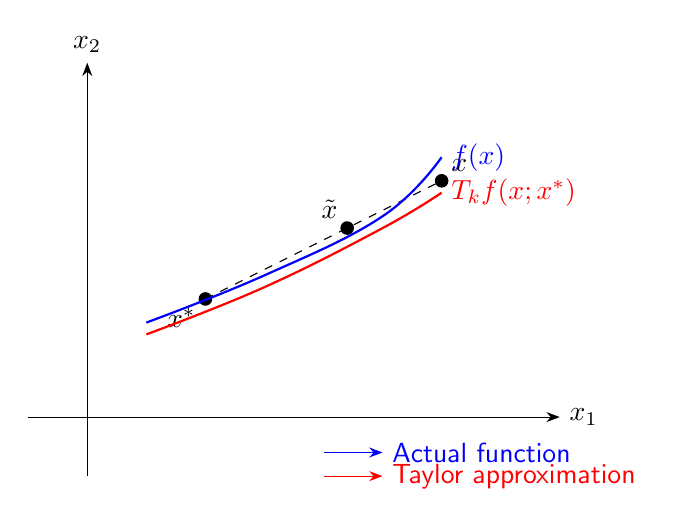
\begin{tikzpicture}[scale=1.5, >=Stealth]
    % Coordinate axes
    \draw[->] (-0.5,0) -- (4,0) node[right]{$x_1$};
    \draw[->] (0,-0.5) -- (0,3) node[above]{$x_2$};
    
    % Points
    \coordinate (xstar) at (1,1);
    \coordinate (x) at (3,2);
    \filldraw (xstar) circle (1.5pt) node[below left]{$x^*$};
    \filldraw (x) circle (1.5pt) node[above right]{$x$};
    
    % Line segment
    \draw[dashed] (xstar) -- (x);
    
    % Function surface
    \draw[blue, thick] plot[smooth, tension=0.7] coordinates {(0.5,0.8) (1.5,1.2) (2.5,1.7) (3,2.2)};
    \node[blue, right] at (3,2.2) {$f(x)$};
    
    % Taylor approximation
    \draw[red, thick] plot[smooth, tension=0.7] coordinates {(0.5,0.7) (1.5,1.1) (2.5,1.6) (3,1.9)};
    \node[red, right] at (3,1.9) {$T_k f(x; x^*)$};
    
    % Intermediate point
    \coordinate (xtilde) at ($(xstar)!0.6!(x)$);
    \filldraw[black] (xtilde) circle (1.5pt) node[above left]{$\tilde{x}$};
    
    % Legend
    \draw[->, blue] (2,-0.3) -- (2.5,-0.3) node[right]{Actual function};
    \draw[->, red] (2,-0.5) -- (2.5,-0.5) node[right]{Taylor approximation};
\end{tikzpicture}
\caption{Visualization of Taylor's theorem in \(\mathbb{R}^2\). The blue curve represents the actual function \( f \), while the red curve shows its \( k \)-th order Taylor approximation \( T_k f \) at \( x^* \). The point \( \tilde{x} \) lies on the line segment between \( x^* \) and \( x \).}
\end{figure}
\newpage
\section{Local Optima of Multivariate Functions}
\end{document}


